\section{HNM AI2: separating two actual finite-profile predictions\workstar}
\subsection{New observables require a new complete support}
Use the free unit cube with origin $(3,1,0)$ and the prescribed physical six-cycle $X$. Let $f_4$ and $f_5$ be the opposite $yz$ faces with anchor sums four and five, and let $Y_r=X\triangle f_r$ be the corresponding simple six-cycles. Define actual character multiplication operators, extended by identity,
\begin{equation}
B_r=(\chi_X+\chi_{Y_r})/\sqrt2,\qquad \psi_r=B_r\Omega,\qquad r=4,5.
\label{r27:eq:probes}
\end{equation}
Each operator is bounded, real, self-adjoint and gauge-invariant. Conditional Haar integration along the common four-link path and the two independent two-link paths gives mean zero, variance one and fourth moment $5/2$. The exact multiplication norm is $J=2\sqrt2$, not one: its triangle upper bound is approached on positive-measure neighborhoods of identity holonomies. A normalized source vector therefore does not authorize replacing its multiplier by a norm-one rank operator.

Each source uses eight free links, but their union has ten. The complete-factor collar must start from that union. For depths $k=0,\ldots,5$, independently reconstructed retained-face counts are
\begin{equation}
N_k=(2,25,143,359,695,1171).
\label{r27:eq:collars}
\end{equation}
The last collar contains 993 reference factors and 1857 complete links. Copying the earlier eight-link seed would omit part of $B_5$. All six cube faces occur by depth one. The inherited AA2 averaged-orbit and exterior-exclusion theorem applies to the entire sixteen-state component containing both sources; it is not an assertion that this component is the entire regional energy shell. The check reconstructs all twenty exterior touching faces and retains their loading and nonzero frequency conditions.

\subsection{From connected words to the full scalar disk}
Each complete reference factor contains at most ten links, each link meets at most four faces, and an interaction adds at most three factors. Counting every ordered connected word, repetition, factor-two commutator and time simplex yields $(10/3)_n/n!$. For $x=15z<1$, a conservative bound on the \emph{whole} omitted series is
\begin{equation}
D_k^{(10)}(x)=\frac{(10/3)_{k+1}}{(k+1)!}\,
\frac{x^{k+1}}{(1-x)^{k+5}}.\workstar
\label{r27:eq:tail}
\end{equation}
Taylor's positive integral remainder has exponent $k+13/3$; rounding it upward to $k+5$ increases the bound. This accounts for paths leaving the collar and returning. It is neither a finite-spin cutoff nor a global propagator-norm statement.

The retained symmetric $16\times16$ matrix $Q(q)$ has physical face-flip entries $q^4$ or $q^5$ and row norm at most six. Set
\begin{equation}
s_q=\frac{3z(1+q)^2(1+q^2)}{p(q)},\qquad v=s_q/96,\qquad
h_r=\langle\psi_r,e^{ivQ(q)}\psi_r\rangle.
\label{r27:eq:center}
\end{equation}
Its exact first moments are $\langle Q\rangle_{\psi_4}=q^4$ and
$\langle Q\rangle_{\psi_5}=q^5$; at $q=1$ both moment lists through degree six equal $(1,1,4,8,32,80,320)$. The computations evaluate rational moments through degree eight. The exponential center error is separately bounded by $(6v)^9/9!$.

The inherited canonical magnetic-profile sum is
$b(q)=p(q)/[24(1-q)^3(1+q)^2(1+q^2)]$. Write
$\tau_q=\eta/[8b(q)]$, $M_k=N_k/24$ and
$\widehat d_q=\tau_q\sqrt{b(q^2)/96}/[(1-\eta)/8]$.
The complete physical-to-center radius is bounded by
\begin{equation}
R_{\mathrm{phys}}=48\widehat d_q+8D_k^{(10)}(15z)
+64\tau_qM_k(1+3zM_k),\qquad
R=R_{\mathrm{phys}}+\frac{(6v)^9}{9!}.\workstar
\label{r27:eq:disk}
\end{equation}
The terms respectively retain the stationary connected-state correction, full spatial tail, both source and vacuum averaging replacements, and arithmetic center error. The constants retain $J^2=8$ and $1+J<4$. A rational upward square-root enclosure controls $\widehat d_q$. Fractions determine the verdicts; decimal values are displays. Omitting multiplier loading, connected-state correction or the returned spatial paths would invalidate the disk.

\subsection{A successful pairwise test and an unsuccessful ratio certificate}
Freeze $z=10^{-6}$ and compare, for each $u\in\{10^{-12},10^{-18},10^{-24}\}$,
\begin{equation}
H_1:(q,\eta)=(1-u,1/2),\qquad H_2:(q,\eta)=(1-2u,1/16).
\label{r27:eq:hypotheses}
\end{equation}
Both satisfy $\eta(1-q)^3=u^3/2$. With common independently fixed $\alpha$, they therefore have the same carrier and the same physical time
\begin{equation}
T=2\cdot10^{-6}u^{-3}\,\hbar/\alpha.
\label{r27:eq:time2}
\end{equation}
For each $k\in\{3,4,5\}$ and probe $r$, compare rational imaginary centers. A positive margin
\begin{equation}
\mathfrak m_r=
\abs{\Impart h_{r,1}^{(8)}-\Impart h_{r,2}^{(8)}}-R_1-R_2>0
\label{r27:eq:margin}
\end{equation}
proves disjoint complex disks and hence distinct actual scalar predictions. Overlap only means this sufficient test failed. It does not establish equality of the two exact models.

Only the cell $u=10^{-18}$, $k=5$ gives a positive margin for either probe. The conservative margins are about $3.21452\times10^{-26}$ for $B_4$ and $4.40500\times10^{-26}$ for $B_5$. Equal additional absolute scalar-error radii must each be strictly below half the relevant margin. Its physical time is $2\times10^{48}\hbar/\alpha$. This is a conditional mathematical distinction between two named hypotheses, not feasible laboratory calibration or an inverse valid on a continuous parameter domain. Timing uncertainty cannot silently be assigned the same scalar-error allowance without a separate sensitivity bound.

The retained coefficient ratio is exactly $q^5/q^4=q$. For actual finite-time values $y_r$, however, spectral calculus first gives
\begin{equation}
\abs{\Impart h_r-vq^r}\le36v^3,\qquad
\abs{y_r-vq^r}\le E_r:=R_r+36v^3.
\label{r27:eq:ratioerror}
\end{equation}
If $vq^4-E_4>0$, interval division yields
\begin{equation}
\frac{vq^5-E_5}{vq^4+E_4}\le\frac{y_5}{y_4}\le
\frac{vq^5+E_5}{vq^4-E_4}.
\label{r27:eq:ratio}
\end{equation}
If the denominator enclosure contains zero, no ratio inference is made. These simple ratio intervals overlap in all nine cells, including the successful scalar-discrimination cell. Their cubic sine-remainder floor is too conservative for that inverse. The result therefore resolves a pairwise scalar question while preserving the failed ratio objective. No derivative of the full-system correlation is inferred from a value-only disk.

\begin{figure}[ht]
\centering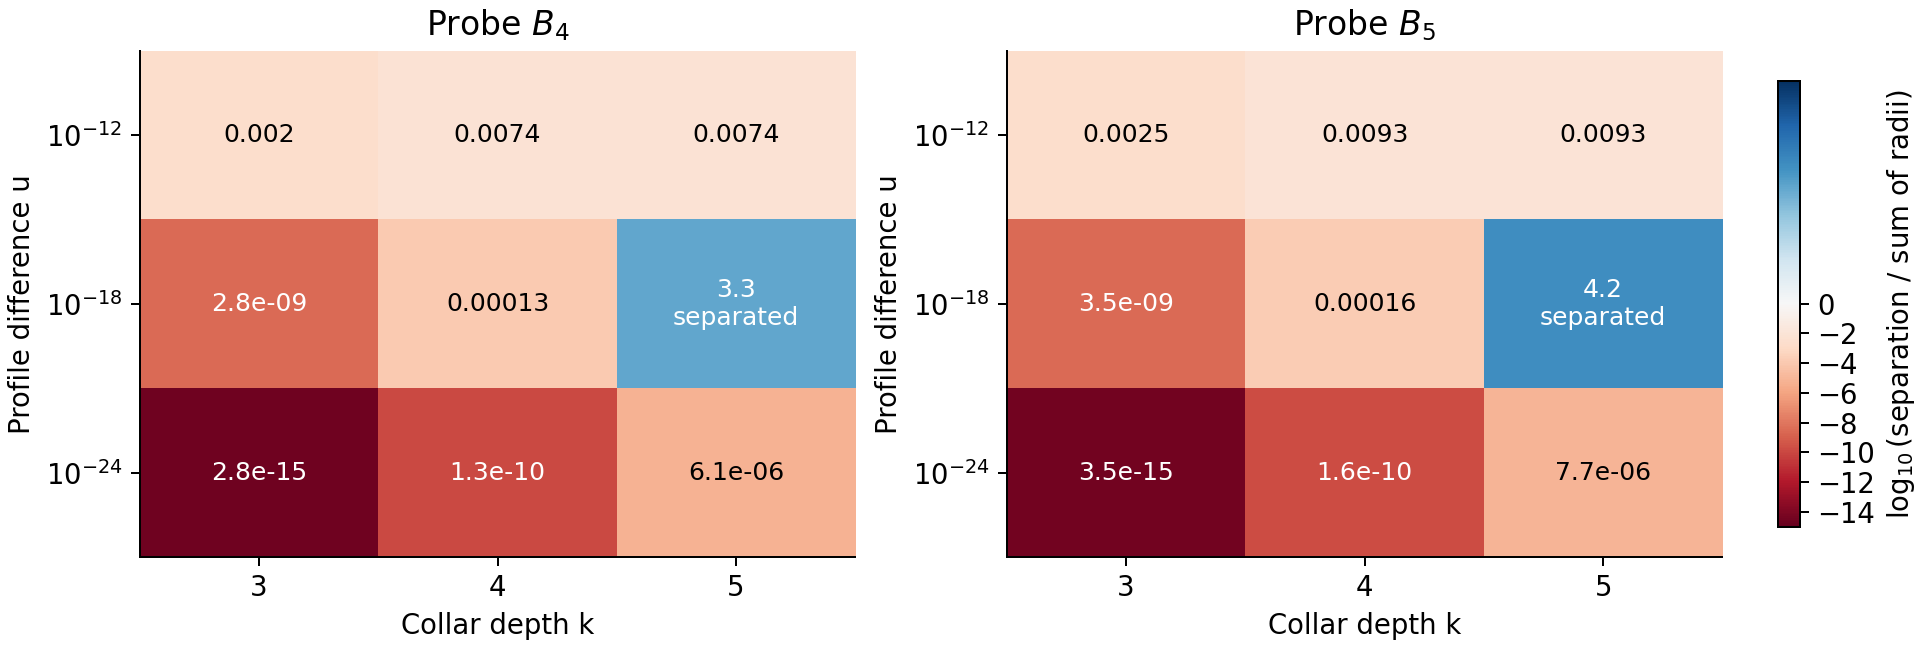
\includegraphics[width=\textwidth]{figures/ym-round27-discrimination.png}
\caption{AI2: separation of imaginary centers divided by the sum of complete radii, computed from exact output fractions. Values above one certify disjoint disks. The only successful grid cell is $u=10^{-18}$, $k=5$ for both probes. Logarithmic color prevents the large failed range from hiding the threshold; the figure is a display of exact decisions, not a numerical proof.}
\label{r27:fig:discrimination}
\end{figure}
